% Options for packages loaded elsewhere
\PassOptionsToPackage{unicode}{hyperref}
\PassOptionsToPackage{hyphens}{url}
\PassOptionsToPackage{dvipsnames,svgnames,x11names}{xcolor}
%
\documentclass[
  a4paper]{article}

\usepackage{amsmath,amssymb}
\usepackage{iftex}
\ifPDFTeX
  \usepackage[T1]{fontenc}
  \usepackage[utf8]{inputenc}
  \usepackage{textcomp} % provide euro and other symbols
\else % if luatex or xetex
  \usepackage{unicode-math}
  \defaultfontfeatures{Scale=MatchLowercase}
  \defaultfontfeatures[\rmfamily]{Ligatures=TeX,Scale=1}
\fi
\usepackage{lmodern}
\ifPDFTeX\else  
    % xetex/luatex font selection
\fi
% Use upquote if available, for straight quotes in verbatim environments
\IfFileExists{upquote.sty}{\usepackage{upquote}}{}
\IfFileExists{microtype.sty}{% use microtype if available
  \usepackage[]{microtype}
  \UseMicrotypeSet[protrusion]{basicmath} % disable protrusion for tt fonts
}{}
\makeatletter
\@ifundefined{KOMAClassName}{% if non-KOMA class
  \IfFileExists{parskip.sty}{%
    \usepackage{parskip}
  }{% else
    \setlength{\parindent}{0pt}
    \setlength{\parskip}{6pt plus 2pt minus 1pt}}
}{% if KOMA class
  \KOMAoptions{parskip=half}}
\makeatother
\usepackage{xcolor}
\usepackage[margin=1in]{geometry}
\setlength{\emergencystretch}{3em} % prevent overfull lines
\setcounter{secnumdepth}{5}
% Make \paragraph and \subparagraph free-standing
\ifx\paragraph\undefined\else
  \let\oldparagraph\paragraph
  \renewcommand{\paragraph}[1]{\oldparagraph{#1}\mbox{}}
\fi
\ifx\subparagraph\undefined\else
  \let\oldsubparagraph\subparagraph
  \renewcommand{\subparagraph}[1]{\oldsubparagraph{#1}\mbox{}}
\fi


\providecommand{\tightlist}{%
  \setlength{\itemsep}{0pt}\setlength{\parskip}{0pt}}\usepackage{longtable,booktabs,array}
\usepackage{calc} % for calculating minipage widths
% Correct order of tables after \paragraph or \subparagraph
\usepackage{etoolbox}
\makeatletter
\patchcmd\longtable{\par}{\if@noskipsec\mbox{}\fi\par}{}{}
\makeatother
% Allow footnotes in longtable head/foot
\IfFileExists{footnotehyper.sty}{\usepackage{footnotehyper}}{\usepackage{footnote}}
\makesavenoteenv{longtable}
\usepackage{graphicx}
\makeatletter
\def\maxwidth{\ifdim\Gin@nat@width>\linewidth\linewidth\else\Gin@nat@width\fi}
\def\maxheight{\ifdim\Gin@nat@height>\textheight\textheight\else\Gin@nat@height\fi}
\makeatother
% Scale images if necessary, so that they will not overflow the page
% margins by default, and it is still possible to overwrite the defaults
% using explicit options in \includegraphics[width, height, ...]{}
\setkeys{Gin}{width=\maxwidth,height=\maxheight,keepaspectratio}
% Set default figure placement to htbp
\makeatletter
\def\fps@figure{htbp}
\makeatother

\makeatletter
\makeatother
\makeatletter
\makeatother
\makeatletter
\@ifpackageloaded{caption}{}{\usepackage{caption}}
\AtBeginDocument{%
\ifdefined\contentsname
  \renewcommand*\contentsname{Table of contents}
\else
  \newcommand\contentsname{Table of contents}
\fi
\ifdefined\listfigurename
  \renewcommand*\listfigurename{List of Figures}
\else
  \newcommand\listfigurename{List of Figures}
\fi
\ifdefined\listtablename
  \renewcommand*\listtablename{List of Tables}
\else
  \newcommand\listtablename{List of Tables}
\fi
\ifdefined\figurename
  \renewcommand*\figurename{Figure}
\else
  \newcommand\figurename{Figure}
\fi
\ifdefined\tablename
  \renewcommand*\tablename{Table}
\else
  \newcommand\tablename{Table}
\fi
}
\@ifpackageloaded{float}{}{\usepackage{float}}
\floatstyle{ruled}
\@ifundefined{c@chapter}{\newfloat{codelisting}{h}{lop}}{\newfloat{codelisting}{h}{lop}[chapter]}
\floatname{codelisting}{Listing}
\newcommand*\listoflistings{\listof{codelisting}{List of Listings}}
\makeatother
\makeatletter
\@ifpackageloaded{caption}{}{\usepackage{caption}}
\@ifpackageloaded{subcaption}{}{\usepackage{subcaption}}
\makeatother
\makeatletter
\@ifpackageloaded{tcolorbox}{}{\usepackage[skins,breakable]{tcolorbox}}
\makeatother
\makeatletter
\@ifundefined{shadecolor}{\definecolor{shadecolor}{rgb}{.97, .97, .97}}
\makeatother
\makeatletter
\makeatother
\makeatletter
\makeatother
\ifLuaTeX
  \usepackage{selnolig}  % disable illegal ligatures
\fi
\IfFileExists{bookmark.sty}{\usepackage{bookmark}}{\usepackage{hyperref}}
\IfFileExists{xurl.sty}{\usepackage{xurl}}{} % add URL line breaks if available
\urlstyle{same} % disable monospaced font for URLs
\hypersetup{
  pdftitle={Timing the Core Equity Factor: Summary},
  pdfauthor={Faune Blanchard},
  colorlinks=true,
  linkcolor={blue},
  filecolor={Maroon},
  citecolor={Blue},
  urlcolor={Blue},
  pdfcreator={LaTeX via pandoc}}

\title{Timing the Core Equity Factor: Summary}
\author{Faune Blanchard}
\date{}

\begin{document}
\maketitle
\ifdefined\Shaded\renewenvironment{Shaded}{\begin{tcolorbox}[boxrule=0pt, frame hidden, borderline west={3pt}{0pt}{shadecolor}, interior hidden, breakable, sharp corners, enhanced]}{\end{tcolorbox}}\fi

\renewcommand*\contentsname{Table of contents}
{
\hypersetup{linkcolor=}
\setcounter{tocdepth}{4}
\tableofcontents
}
\newpage

\hypertarget{introduction}{%
\section{Introduction}\label{introduction}}

This report summarizes our analysis of European equity returns to time
the core equity factor. We used Principal Component Analysis (PCA) to
extract the first latent factor, evaluated the replicating portfolio's
alpha, and examined the performance of a long/flat investment strategy
derived from the portfolio's slope trends.

\hypertarget{part-1-principal-component-analysis-pca}{%
\section{Part 1: Principal Component Analysis
(PCA)}\label{part-1-principal-component-analysis-pca}}

To extract the core factor, we applied PCA to the European equity
returns and identified the first latent factor, denoted as \(F_1\). This
factor was rescaled to match the benchmark's volatility. Additionally,
we adjusted the sign of \(F_1\) to ensure a positive correlation with
stock returns.

We estimated the sensitivities of individual stocks to \(F_1\) using a
linear regression model. The equation used for this estimation was:
\[r_{i,t} = \alpha_i + \hat{b}_{1,i} F_{1,t} + \varepsilon_t.\]

The beta values of individual stocks to the core factor vary
significantly, as shown in the beta distribution plot:

\begin{figure}

{\centering 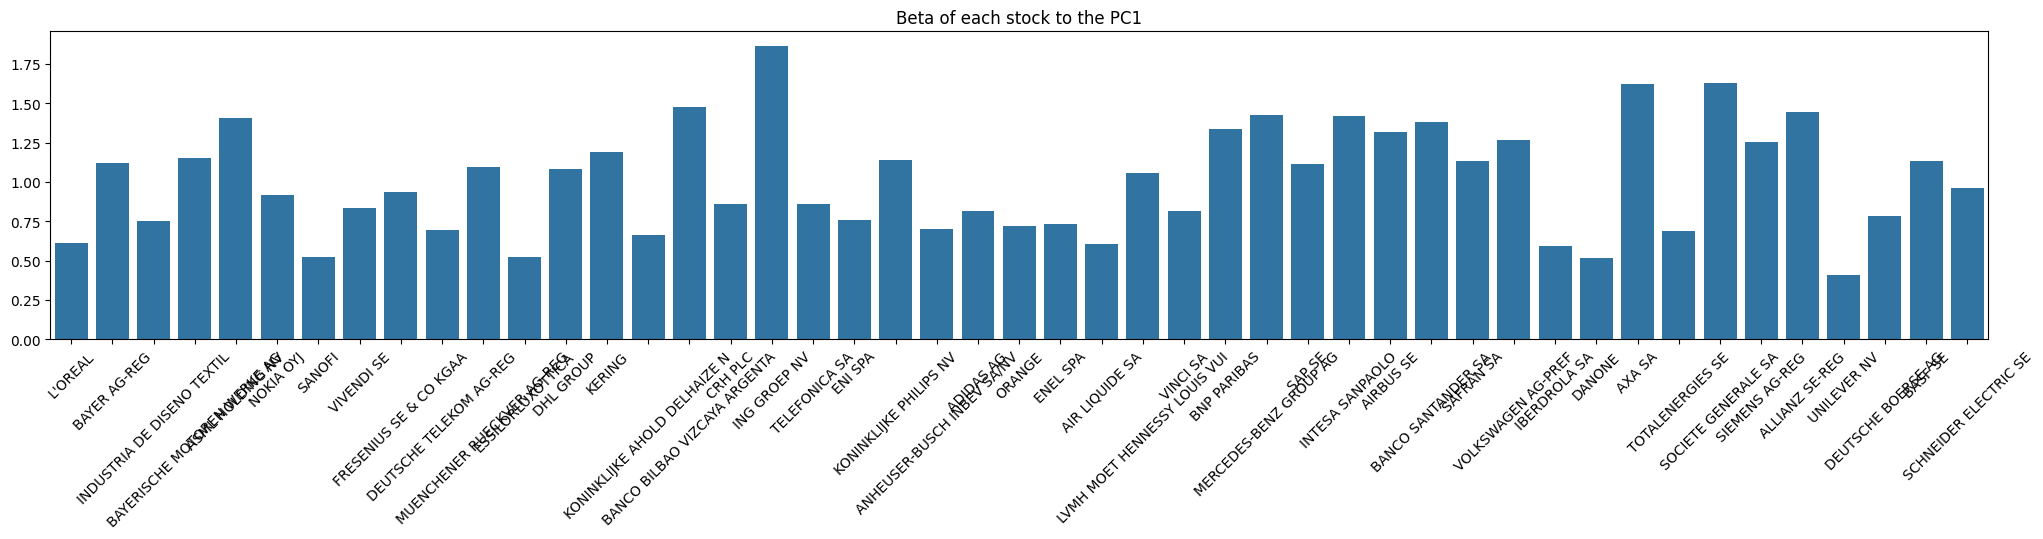
\includegraphics[width=1\textwidth,height=\textheight]{C:/Users/faune/core-equity-factors/graphs/beta_stocks_pc1.png}

}

\caption{Beta of each stock to the PC1}

\end{figure}

This variability reflects differences in their alignment with the core
equity factor.

Subsequently, we constructed a replicating portfolio for \(F_1\) by
optimizing the portfolio weights to minimize variance. This optimization
was carried out under the constraints of maintaining a unitary
sensitivity to \(F_1\), ensuring non-negative weights, and setting the
total weight to one. We end up with a rougly equally weighted portfolio.

\begin{figure}

{\centering 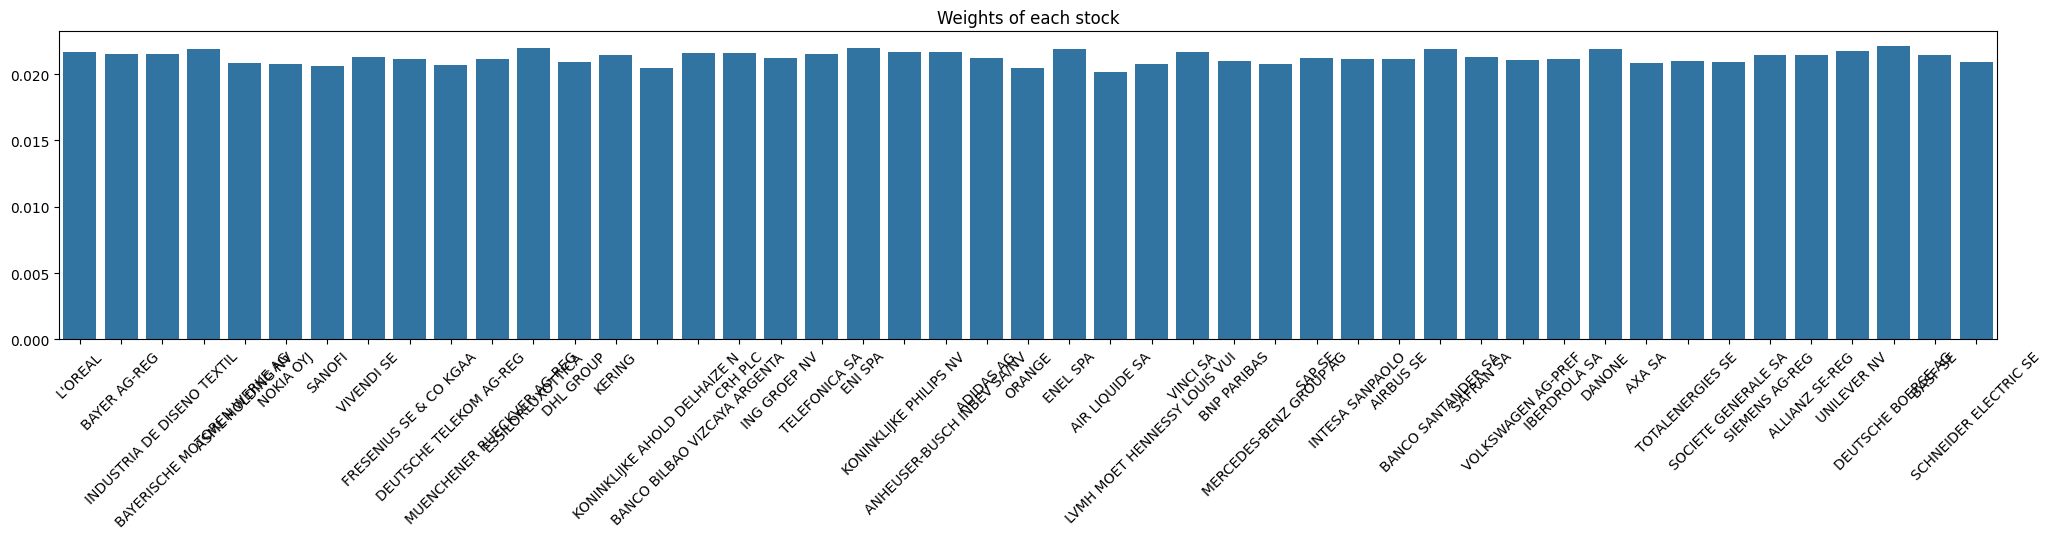
\includegraphics[width=1\textwidth,height=\textheight]{C:/Users/faune/core-equity-factors/graphs/weights_ptf.png}

}

\caption{Weight of each stock in the Replicating portfolio}

\end{figure}

\newpage

\hypertarget{part-2-portfolio-alpha-and-confidence-analysis}{%
\section{Part 2: Portfolio Alpha and Confidence
Analysis}\label{part-2-portfolio-alpha-and-confidence-analysis}}

The replicating portfolio we designed demonstrated a neutral alpha when
compared to the Eurostoxx 50 index, indicating its potential to
replicate the benchmark. We assessed the impact of estimation errors in
the covariance matrix on this alpha by employing a bootstrap
methodology. This approach allowed us to estimate the 95\% confidence
interval for the alpha and address biases introduced by sample
covariance errors.

We visualized the strategy's alpha and its confidence interval:

\begin{figure}

{\centering 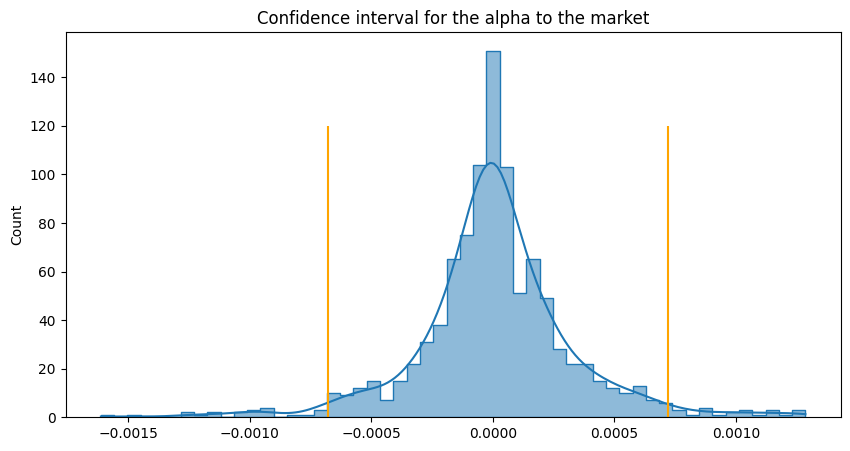
\includegraphics[width=0.7\textwidth,height=\textheight]{C:/Users/faune/core-equity-factors/graphs/alpha_market.png}

}

\caption{Bootstrapped Alphas}

\end{figure}

The orange lines in the plot represent the confidence intervals,
highlighting that the strategy's alpha is centered around 0, replicating
the index.

\newpage

\hypertarget{part-3-investment-strategy}{%
\section{Part 3: Investment Strategy}\label{part-3-investment-strategy}}

To further analyze the replicating portfolio, we estimated its price
index, \(I_{1,t}\), using a local linear trend model. This model enabled
us to decompose the price index into its trend component, \(T_{1,t}\),
and slope, \(S_{1,t}\). We then derived an investment strategy based on
the slope's behavior. Specifically, when \(S_{1,t-1}\) was greater than
zero, we allocated to the replicating portfolio. Conversely, when
\(S_{1,t-1}\) was less than or equal to zero, we allocated to cash at a
constant 3\% annual risk-free rate.

We recoded the kalman filter and got this output:

\begin{figure}

{\centering 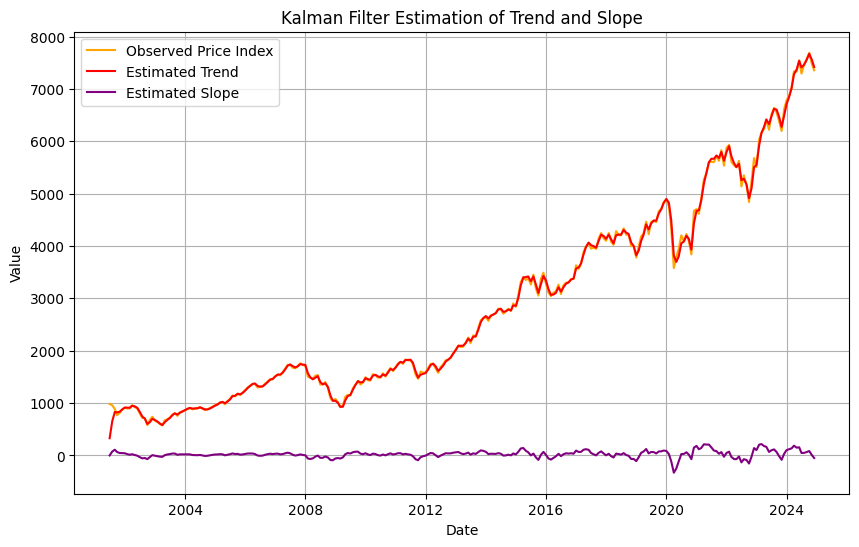
\includegraphics[width=0.7\textwidth,height=\textheight]{C:/Users/faune/core-equity-factors/graphs/kalman_output.png}

}

\caption{Kalman Filter Output}

\end{figure}

In price, this is how the strategy performed compared to the benchmark:

\begin{figure}

{\centering 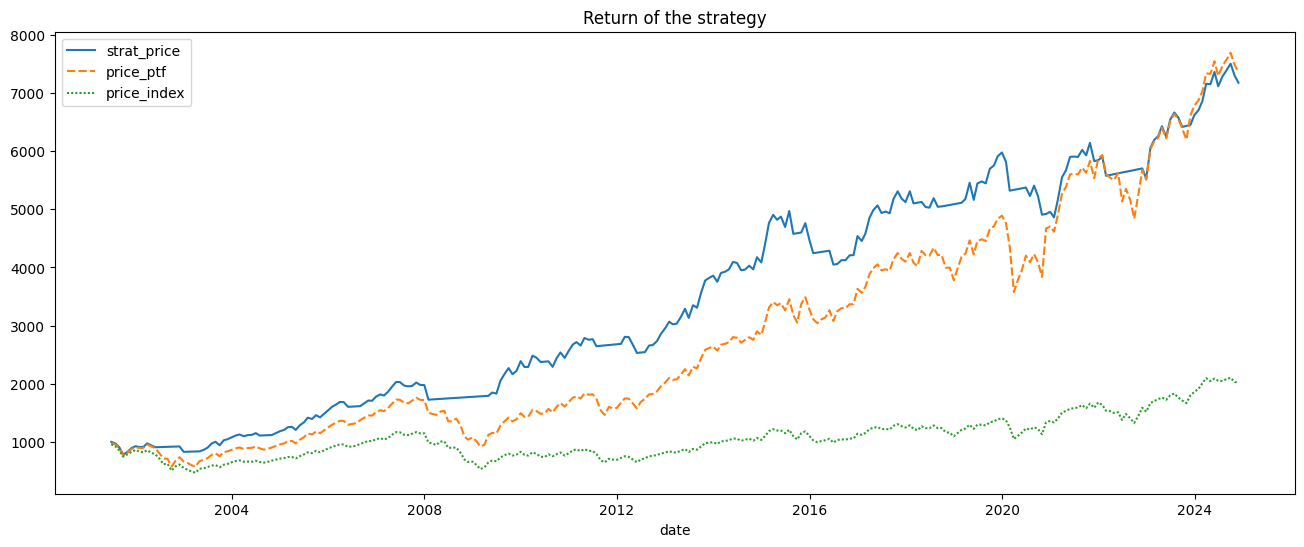
\includegraphics[width=0.7\textwidth,height=\textheight]{C:/Users/faune/core-equity-factors/graphs/return_strat.png}

}

\caption{Performance of the Strategy vs Benchmark}

\end{figure}

\newpage

To evaluate the effectiveness of this strategy, we tested whether its
Sharpe ratio was due to luck or if it was statistically significant. The
performance of the strategy turned out to be mostly insignificant and
due to luck, according to our analysis using sharpe ratios from
long/flat strategies that decided whether to invest in the portfolio or
not at random.

\begin{figure}

{\centering 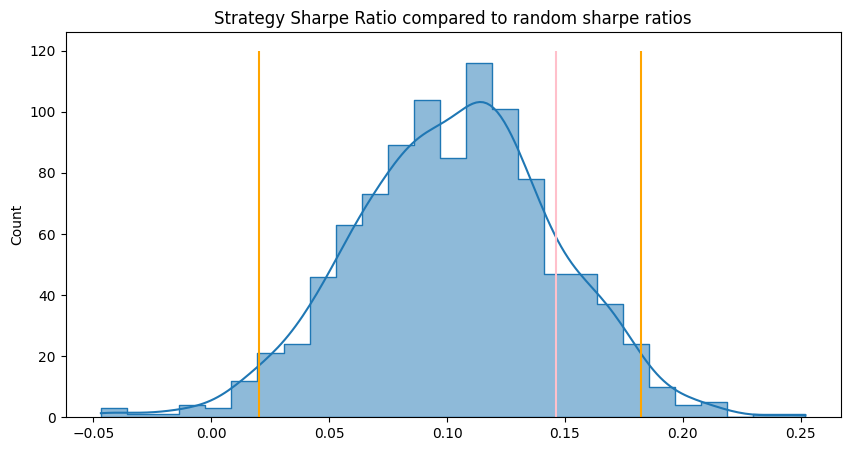
\includegraphics[width=0.7\textwidth,height=\textheight]{C:/Users/faune/core-equity-factors/graphs/sharpe_ratios.png}

}

\caption{Randomized Sharpe Ratios}

\end{figure}

\hypertarget{conclusion}{%
\section{Conclusion}\label{conclusion}}

Our analysis underscores the utility of PCA for identifying core equity
factors and constructing replicating portfolios. The replicating
portfolio's positive alpha and statistically significant Sharpe ratio
demonstrate the practicality of these techniques in timing equity
factors. Future work could explore dynamic weighting schemes to enhance
the portfolio's robustness in varying market conditions.



\end{document}
